\section{Bounded supports and uniform arithmetic}

Let \(f:\mathcal Y\to S\) be smooth and projective, of relative
dimension \(n\), where \(S\) is a smooth irreducible complex algebraic
variety. Fix a relatively very ample line bundle \(L\), an integer
\(0\le p\le n\), and a global flat section
\[
 \gamma\in H^0(S,R^{2p}f_*\Q).
\]
The section may in particular be a flat Hodge class. Degree is measured
using \(L_s\), and cycle classes are in rational cohomology.
Write \(b=\dim_\Q H^{2p}(\mathcal Y_s,\Q)\).

\begin{definition}
For an integer \(D\ge1\), let \(\Sigma_D(\gamma)\) be the set of \(s\in S\) for
which \(\gamma_s\) belongs to the rational span of the classes of
integral codimension-\(p\) subvarieties of degree at most \(D\).
Let \(\Sigma(\gamma)=\bigcup_{D\ge1}\Sigma_D(\gamma)\).
\end{definition}

\begin{theorem}[Closedness and automatic denominators]
\label{v7:new:thm:degree-closed}
For each \(D\), the locus \(\Sigma_D(\gamma)\) is Zariski closed.
There are integers \(N_D>0\) and \(D'_D\ge0\) such that, at every
\(s\in\Sigma_D(\gamma)\), there are effective integral cycles
\(Z_s^+\) and \(Z_s^-\) of codimension \(p\) satisfying
\[
 N_D\gamma_s=[Z_s^+]-[Z_s^-],\qquad
 \deg_L Z_s^+,\ \deg_L Z_s^-\le D'_D.
\]
Thus no separate uniform denominator hypothesis is needed once the
degrees of the supports are bounded.
\end{theorem}

\begin{proof}
Any spanning collection can be reduced to at most \(b\) classes.
For each \(1\le r\le b\) and each degree tuple
\((d_1,\ldots,d_r)\in\{1,\ldots,D\}^r\), take the product over \(S\)
of the relative Chow spaces of effective cycles of these degrees.
These are projective \(S\)-schemes of finite type, with finitely many
connected components. Only finitely many parameter spaces occur.
The standard construction and specialization of algebraic cycles
are as in \cite{Ful98}.

On a connected parameter component \(T\), the classes
\(v_1,\ldots,v_r\) of the ordered universal cycles are flat sections
of the pulled-back local system. Hence the condition
\[
 \gamma=\sum_{i=1}^r q_i v_i\quad(q_i\in\Q)
\]
holds somewhere on \(T\) if and only if it holds everywhere on \(T\)
with the same coefficients. The same conclusion follows by normalizing
components and specialization if the Chow space is singular.
The image of each admissible component is closed, because the
parameter morphism is proper. The finite union of these images is
\(\Sigma_D(\gamma)\). Parameterizing effective cycles rather than
integral subvarieties changes nothing: every irreducible component
of a cycle of degree at most \(D\) has degree at most \(D\).

Choose one coefficient tuple in the displayed span relation for each nonempty admissible
component. There are finitely many choices. Let \(N_D\) clear all
their denominators, and let \(A_D\) bound all the absolute integer
coefficients \(N_Dq_i\). Splitting the resulting combination into
its positive and negative parts proves the displayed signed-cycle bounds, with
\(D'_D=bD A_D\). If \(\gamma=0\), the empty cycles suffice.
\end{proof}

\begin{remark}
The proof gives existence of \(N_D,D'_D\), not an effective bound
from the numerical degree \(D\) alone. The coefficients are selected
on the finitely many actual Chow components.
\end{remark}

\section{A global cycle from one dominating component}

\begin{theorem}[Equivalent propagation criteria]
\label{v7:new:thm:global}
The following conditions are equivalent.
\begin{enumerate}
\item \(\Sigma(\gamma)\) is nonmeagre in the complex analytic topology.
\item \(\Sigma(\gamma)=S\).
\item For some \(D\), \(\Sigma_D(\gamma)\) is Zariski dense in \(S\).
\item For some \(D\), \(\Sigma_D(\gamma)=S\).
\item There is \(z\in\CH^p(\mathcal Y)_\Q\) whose cohomological
restriction to every fibre is \(\gamma_s\).
\item There are fixed \(N>0,D'>0\) for which the displayed signed-cycle bounds hold at every \(s\).
\end{enumerate}
In particular, a Zariski dense bounded-degree locus supplies an
actual total-space algebraic cycle, not just separate cycles on
each fibre.
\end{theorem}

\begin{proof}
Theorem~\ref{v7:new:thm:degree-closed} gives \(3\Rightarrow4\Rightarrow6\).
Clearly \(6\Rightarrow4\Rightarrow2\Rightarrow1\).
Also \(5\Rightarrow2\), by compatibility of the cycle-class map with
refined pullback to a smooth fibre.

For \(1\Rightarrow4\), use the countable Hilbert-scheme description
of \(\Sigma(\gamma)\). For each tuple of Hilbert polynomials and
each tuple of rational coefficients, the components satisfying
the cycle-class equality have closed images because the parameter morphisms are proper. There are
countably many such images. If all were proper subsets of \(S\),
their union would be meagre. Therefore one admissible parameter
component dominates \(S\). Its fixed Hilbert polynomials bound the
degrees of all supports in the displayed representatives, and
properness makes its image all of \(S\). This proves condition 4.

It remains to prove \(4\Rightarrow5\). Use one irreducible admissible
Chow component \(T\to S\) that dominates \(S\); one exists because a
finite union of proper closed subsets cannot cover the irreducible
base. Let \(K=\mathbb C(S)\). The nonempty generic fibre \(T_K\)
has a closed point with residue field a finite extension \(K'/K\).
The cycles at that point, with their fixed coefficients, define
\(\zeta_{K'}\in\CH^p(\mathcal Y_{K'})_\Q\).

Spread this point and these cycles over a sufficiently small dense
open subset of the normalization of \(S\) in \(K'\). Shrink the
base so that the finite cover is etale and the cycles are flat.
Every geometric fibre of the spread represents the pullback of
\(\gamma\). Proper pushforward along the finite cover, divided by
\([K':K]\), therefore gives a rational cycle on \(\mathcal Y\) over
that open subset whose fibre class is \(\gamma\).

Take the closures of its finitely many components in \(\mathcal Y\).
They retain codimension \(p\). Their cohomology class restricts to
a flat section of \(R^{2p}f_*\Q\). This section agrees with
\(\gamma\) on a nonempty open subset and hence everywhere, because
\(S\) is connected. Refined pullback to any fibre gives the claimed
rational algebraic representative there.
\end{proof}

\begin{figure}[ht]
\centering
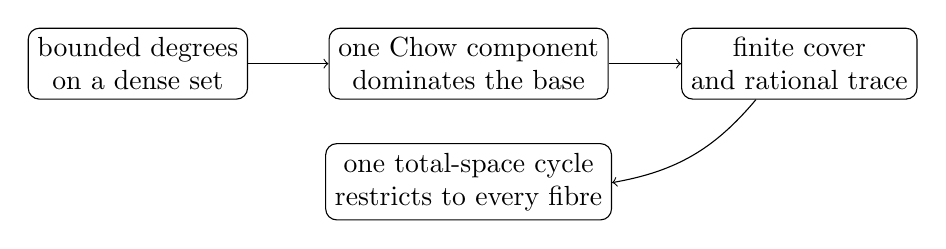
\begin{tikzpicture}[x=1cm,y=1cm]
\node[draw,rounded corners,align=center] (a) at (0,0)
 {bounded degrees\\on a dense set};
\node[draw,rounded corners,align=center] (b) at (4.2,0)
 {one Chow component\\dominates the base};
\node[draw,rounded corners,align=center] (c) at (8.4,0)
 {finite cover\\and rational trace};
\node[draw,rounded corners,align=center] (d) at (4.2,-1.5)
 {one total-space cycle\\restricts to every fibre};
\draw[->] (a)--(b);
\draw[->] (b)--(c);
\draw[->] (c) to[bend left=20] (d);
\end{tikzpicture}
\caption{Proper parameter spaces convert a uniform geometric
complexity bound into a global algebraic cycle. Density alone
does not provide the bound.}
\end{figure}

\begin{corollary}[Complexity on a curve]
\label{v7:new:cor:escape}
Suppose \(S\) is a curve and \(\Sigma(\gamma)\ne S\). Then
\(\Sigma_D(\gamma)\) is finite for every \(D\). Consequently, if
\(s_1,s_2,\ldots\) are distinct points of \(\Sigma(\gamma)\), the
smallest support-degree bound needed to span \(\gamma_{s_j}\)
tends to infinity.
On a curve algebraicity at an uncountable set of fibres suffices
for all the conditions of Theorem~\ref{v7:new:thm:global}.
\end{corollary}

\begin{proof}
Each \(\Sigma_D\) is a proper closed subset of a curve, hence finite.
Every fixed \(D\) therefore occurs at only finitely many terms of the
sequence. The union over \(D\) is countable unless it is all of \(S\).
\end{proof}

\section{A weaker test using one detected support}

The next criterion avoids requiring the target class itself to lie
in the span of the bounded-degree supports. Its constant-subsystem
hypothesis is essential to prevent cancellation under trace.

\begin{theorem}[Bounded-degree detection]
\label{v7:new:thm:detection}
Assume that a relative rational algebraic correspondence gives a flat
projector \(\Pi\) on \(R^{2p}f_*\Q\). Let \(W\) be a constant rational
sub-local system of \(\operatorname{im}\Pi\). Assume that at every
very general fibre,
\[
 \Pi\bigl(\Hdg^p(\mathcal Y_s)\bigr)\subseteq W_s.
\]
Suppose that for some \(D\), at a Zariski dense set of points \(s\)
there is an integral codimension-\(p\) subvariety \(V_s\), of degree
at most \(D\), with \(\Pi_s[V_s]\ne0\). Then there is a nonzero
global flat section \(w\) of \(W\), algebraic on every fibre and
represented by a relative total-space rational cycle.
\end{theorem}

\begin{proof}
For each degree at most \(D\), parameterize effective cycles by the
relative Chow variety. On each connected component, vanishing of
the projected cycle class is a flat, hence componentwise, condition.
The images of components on which it is nonzero are finitely many
closed subsets. The hypothesis makes their union dense, so one
irreducible such component \(T\) dominates \(S\).

Choose a point over a very general fibre. By the generic-image hypothesis its projected class
belongs to \(W\). Flatness makes membership in \(W\), and nonvanishing,
valid everywhere on \(T\). Since \(W\) is constant and \(T\) connected,
the projected class is a single fixed nonzero vector \(w\in W\).

Take a finite generic multisection and trace its cycle as in
Theorem~\ref{v7:new:thm:global}. After applying the algebraic projector,
every conjugate has class \(w\), so the trace has class
\([K':K]w\), not zero. Divide by the degree and close up.
The resulting total-space cycle represents \(w\) on every fibre.
\end{proof}

\begin{remark}
For a nonconstant local system, conjugate projected classes can sum
to zero. Nonvanishing at one point alone would not justify the trace
step. The generic-image hypothesis and the constancy of \(W\) are the additional
information used here.
\end{remark}

\subsection*{Application to the matched Mumford mixed class}

In the full-v7 notation, let
\[
 \mathcal Y=\mathcal X\times_S\mathcal X\times_S\mathcal Z,\qquad
 \Pi=\pi_1^{\mathcal X}\otimes\pi_1^{\mathcal X}
                         \otimes\pi_{T_Z}.
\]
Here \(\pi_1\) is the degree-one projector and \(\pi_{T_Z}\) is the
algebraic degree-two projector onto the rank-nine adjoint summand.
Their relative versions are available after the common finite level
cover used to define the two abelian schemes:
\begin{itemize}
\item interpolation in multiplication by two supplies relative
degree projectors;
\item a fixed element of the right norm-one torus supplies the
relative neutral-weight projector;
\item the Tate classes to be subtracted are generated by fixed
right-\(F\) pullbacks of a relative polarization, and their constant
intersection matrix supplies the relative divisor projector.
\end{itemize}
For the last item, squares span \(F\) over \(\Q\), since
\(u=((u+1)^2-(u-1)^2)/4\). Thus finitely many right-\(F\)
endomorphisms suffice. Their divisor classes and rational dual
intersection matrix are algebraic over the same level cover.

At a full-group fibre, the Hodge classes in the image of \(\Pi\)
are exactly
\[
 W=F\xi.
\]
Indeed \(T_X\) has multiplicity one in \(H^1(X)\otimes H^1(X)\),
\(T_Z\) is its irreducible rank-nine partner, and the commuting
field is \(F\). Both summands vary through the same left group,
so this is a constant rank-three rational subsystem.

Consequently, if one can find a fixed \(D\) and infinitely many
distinct fibres carrying one degree-\(\le D\) codimension-two
support with nonzero mixed projection, Theorem~\ref{v7:new:thm:detection}
produces a global class \(e\xi\), with \(0\ne e\in F\).
The already constructed algebraic \(F\)-action on \(T_Z\) applies
\(e^{-1}\) and produces \(\xi\) itself. The full-group transfer
theorem then gives every Hodge class on every power of \(X\) at
such a fibre.

The matched CM construction proves that some support with nonzero
mixed projection exists at each point of its isogeny orbit.
It does not bound the degrees of these supports uniformly.
Theorem~\ref{v7:new:thm:detection} weakens the required geometric input,
but does not supply it. It does not prove the universal statements
F2 or F3'.
